\documentclass[border={10pt 5pt 5pt 5pt},tikz]{standalone}

\usepackage[T1]{fontenc}
\usepackage[sfdefault,scaled=.85]{FiraSans}
\usepackage{tikz}
\usepackage{pgfplots}
\usepackage{ifthen}
\usetikzlibrary{arrows.meta}
\usetikzlibrary{shapes.geometric}
\usetikzlibrary{mindmap,trees,shadows}

\pgfplotsset{compat=1.16}

\usetikzlibrary{arrows.meta,angles,quotes}
\colorlet{linecol}{black!75}
\usepackage{forest}

% Information boxes (from : https://texample.net/tikz/examples/servers/)
\newcommand*{\info}[4][4]{%
  \node [ annotation, #3, scale=1.5, text width = #1em,
          inner sep = 1mm ] at (#2) {%
  \list{$\bullet$}{\topsep=0pt\itemsep=0pt\parsep=0pt
    \parskip=0pt\labelwidth=8pt\leftmargin=8pt
    \itemindent=-5pt\labelsep=2pt}%
    #4
  \endlist
  };
}


\begin{document}

	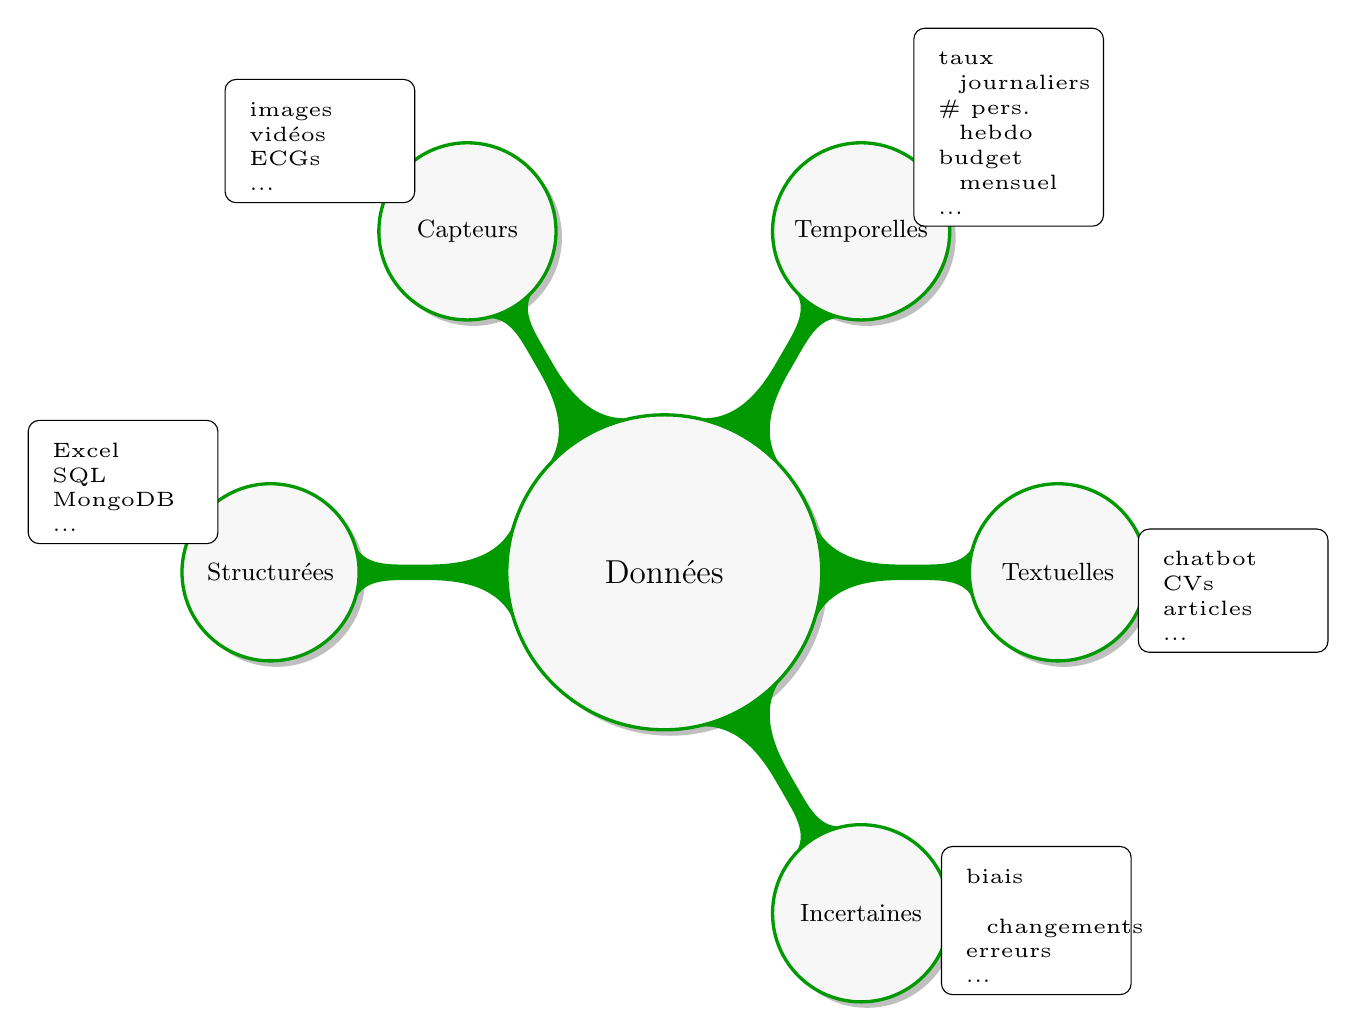
\begin{tikzpicture}[every annotation/.style = {draw, fill = white}]
		\tikzset{concept/.append style={fill={black!3},drop shadow}}
		\path[mindmap,concept color=green!60!black,text=black]
		node[concept] {Données}
			[clockwise from=180]
			child { node[concept] (tab) {Structurées} }
			child { node[concept] (capt) {Capteurs} }
			child { node[concept] (temp) {Temporelles} }
			child { node[concept] (text) {Textuelles} }
			child { node[concept] (datunc) {Incertaines} }
		;
		\info{tab.north west}{above,anchor=east,xshift=1em,yshift=1em}{%
		\item[] Excel
		\item[] SQL
		\item[] MongoDB
		\item[] ...
		}
		\info{capt.north west}{above,anchor=east,xshift=1em,yshift=1em}{%
		\item[] images
		\item[] vidéos
		\item[] ECGs
		\item[] ...
		}
		\info{temp.north east}{above,anchor=west,xshift=-1em,yshift=1.5em}{%
		\item[] taux journaliers
		\item[] \# pers. hebdo
		\item[] budget mensuel
		\item[] ...
		}
		\info{text.south east}{above,anchor=west,yshift=1.6em}{%
		\item[] chatbot
		\item[] CVs
		\item[] articles
		\item[] ...
		}
		\info{datunc.south east}{above,anchor=west,yshift=2em}{%
		\item[] biais
		\item[] changements
		\item[] erreurs
		\item[] ...
		}
\end{tikzpicture}

\end{document}
